\chapter{Implementación}
\label{cap:implementacion}

\chapterquote{Puede que tengas grandes ideas en la cabeza, pero lo que importa es la acción. Una idea, si no se lleva a cabo, no producirá ninguna manifestación, ni resultados ni recompensas}{Miguel Ruiz}


En este capítulo hacemos una descripción detallada sobre la arquitectura de nuestro asistente. Hablaremos también sobre la implementación de las distintas funcionalidades que se ha llevado a cabo tanto en la parte del servidor como en la aplicación en sí.


\section{Arquitectura}

La estructura de nuestro proyecto está soportada sobre un entorno Flask, teniendo el nivel de directorios que se muestra en la Figura \ref{fig:projectStructure}. En las posteriores subsecciones describimos la parte de implementación correspondiente al servidor, explicando tanto los servicios externos utilizados como la librería spaCy, fundamentales para llevar a cabo las funcionalidades que requiere el asistente.

	 \begin{figure}[h!]
	\centering
	
	
	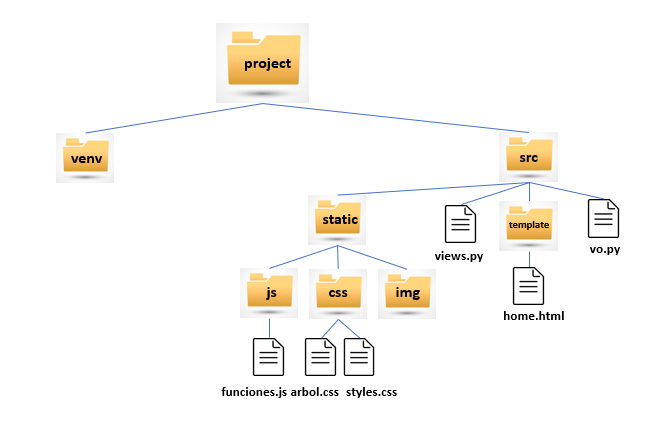
\includegraphics[scale=1.2]{Imagenes/Figuras/Project-Structure}
	
	
	\caption{Estructura del proyecto en Flask}
	\label{fig:projectStructure}
\end{figure}

A continuación, se explican la función de cada uno de los ficheros que componen la aplicación web.

\subsection{Ficheros del entorno}

Los ficheros principales son:
\begin{itemize}
	\item \textbf{views.py}: es el encargado de la lógica de todos los endpoints de la aplicación, así como el renderizado de la plantilla (home.html). Cada una de esas rutas tendrá una funcionalidad distinta, las cuales serán llamadas por una función del archivo de funciones.js dependiendo de la acción que se elija.
	\item \textbf{vo.py}: se encarga de la organización de clases que puedan ser necesarias para la aplicación. En este caso la utilizaremos para definir la clase de cada nodo del árbol de dependencias.
	\item \textbf{home.html}: es la plantilla donde se mostrará el contenido del asistente y con el que el usuario interactuará. En esencia, lo que percibe el usuario por medio de la vista.
	\item \textbf{funciones.js}: la misión de este fichero es comunicar la aplicación web con los elementos del DOM de la misma, haciendo posible la modificación del HTML dinámicamente. Las modificaciones que efectuamos en este archivo es añadir nuevas etiquetas, modificando o eliminando otras, cambiar sus atributos, añadiendo clases, cambiar el contenido de texto, etc. También es el encargado de la comunicación con la vista (views.py) para la petición y respuesta de servicios web.
	\item \textbf{arbol.css}: archivo encargado de generar los estilos para que nuestro árbol de dependencias tenga la apariencia de un árbol genealógico.
	\item \textbf{style.css}: fichero encargado de dar estilos ( (fuentes, disposición, tamaños, colores, etc.) a todo lo que concierne a nuestra aplicación web excepto el árbol de dependencias que tiene sus estilos especiales en ``arbol.css''. 
\end{itemize}

 Todos estos ficheros se encuentran alojados en el repositorio \url{https://github.com/NILGroup/TFG-2021-AsistenteSimplificacion} junto con el resto de directorios del proyecto.

\subsection{Servicios web externos}\label{sec:serviciosWebExternos}
Para hacer uso de las principales funcionalidades descritas en el capítulo \ref{cap:asistenteWeb}, contamos con una arquitectura de servicios web REST basada en endpoints (\textit{URIs}), intercambiando mensajes entre cliente y servidor (Figura \ref{fig:apiRest}). 

\begin{figure}[h!]
	\centering
	
	
	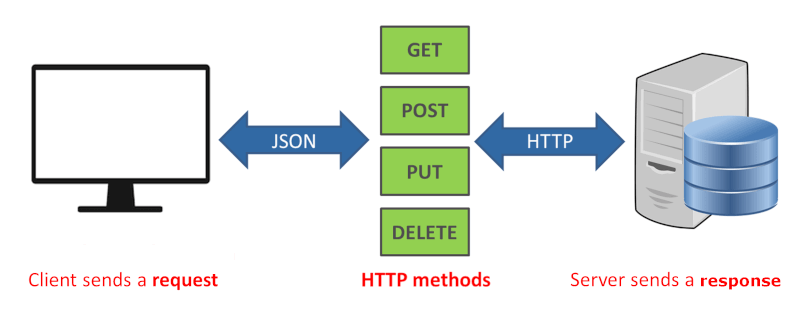
\includegraphics[scale=0.4]{Imagenes/Figuras/rest_api}
	
	
	\caption{Servicio REST cliente/servidor}
	\label{fig:apiRest}
\end{figure}

Un servicio web REST es una interfaz para conectar varios servicios web basados en el protocolo HTTP que define una gran cantidad de métodos. A continuación, describimos los cuatro más básicos:
\begin{itemize}
	\item \textbf{GET}: se utiliza para acceder a los distintos recursos. Si requiere del envío de un parámetro al servidor (\textit{URI param}), éste se pasa como un elemento en la URI (del inglés, \textit{Uniform Resource Identifier}). 
	
	\item \textbf{POST}: se usa para realizar acciones de creación de nuevos recursos. Si se requiere el envío de información al servidor, esta se pasa dentro del cuerpo de la petición HTTP (\textit{body param}).
	
	\item \textbf{PUT}: se utiliza para la modificación de los recursos existentes. Puede enviar parámetros tanto en la URI como en el cuerpo de la petición HTTP.
	
	\item \textbf{DELETE}: se utiliza para la eliminar los recursos existentes, siendo la operación análoga al POST. El parámetro será informado a través de la URI.
\end{itemize}

Estos métodos pueden ser usados en distintas situaciones devolviendo los datos en distintos formatos como XML y JSON.
En nuestro caso, hemos usado el formato JSON.

Nuestra arquitectura REST tiene el aspecto como muestra la Figura \ref{fig:ArquitecturaAsistenteR}. A continuación hablaremos de los diferentes servicios web externos que ofrece la NIL-WS-API y de la librería spaCy que integramos en los distintos endpoints.
\begin{figure}[h!]
	\centering
	
	
	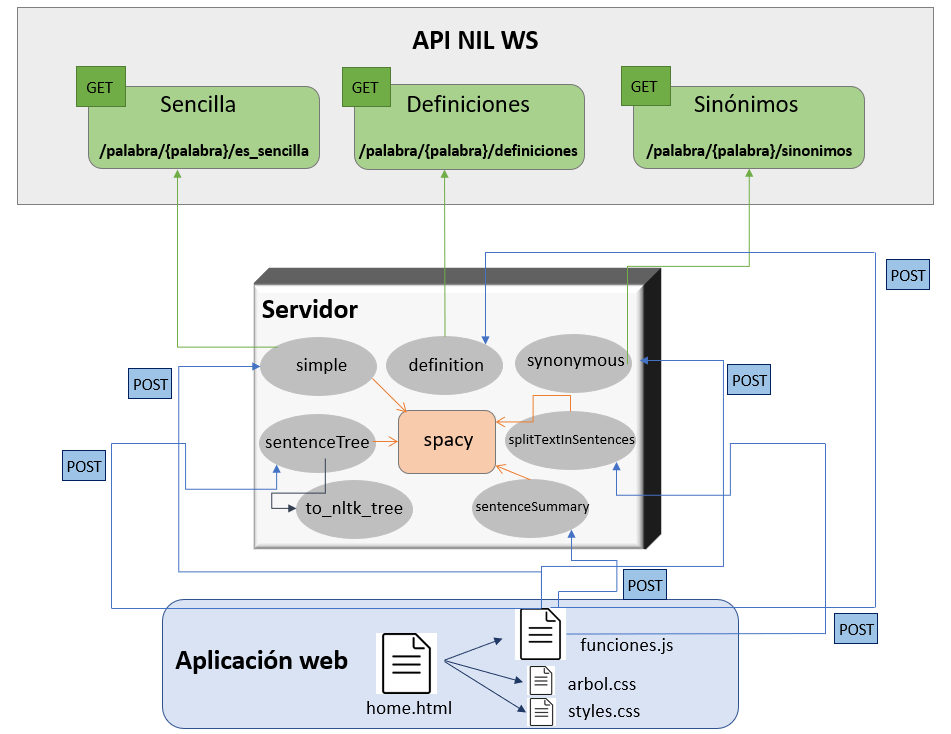
\includegraphics[scale=0.9]{Imagenes/Figuras/ArquitecturaAsistenteR}
	
	
	\caption{Diagrama de la arquitectura REST del asistente web}
	\label{fig:ArquitecturaAsistenteR}
\end{figure}

  Hacemos uso de los siguientes servicios REST que nos ofrece la API del grupo NIL\footnote{Para más información acceder a \href{https://holstein.fdi.ucm.es/nil-ws-api/}{https://holstein.fdi.ucm.es/nil-ws-api/}} descrita en el capítulo \ref{cap:herramientas}, sección \ref{sec:nilws}:


	


\begin{itemize}
	\item \textbf{Servicio para comprobar si una palabra es sencilla}.
	\begin{lstlisting}[backgroundcolor = \color{pink},
	xleftmargin = 1cm,
	framexleftmargin = 1em,frame=tlbr,framesep=4pt,framerule=1pt]
	GET https://holstein.fdi.ucm.es/nil-ws-api/
	palabra/{palabra}/es\_sencilla
	
	
\end{lstlisting}
	
	Este recurso devuelve un objeto en formato JSON que contiene el campo ``palabraSencilla'' de tipo booleano, que en el caso que sea False la palabra introducida a través de la URI es compleja (ver Figura \ref{fig:apiSencilla}).
		 \begin{figure}[h!]
		\centering
		
		
		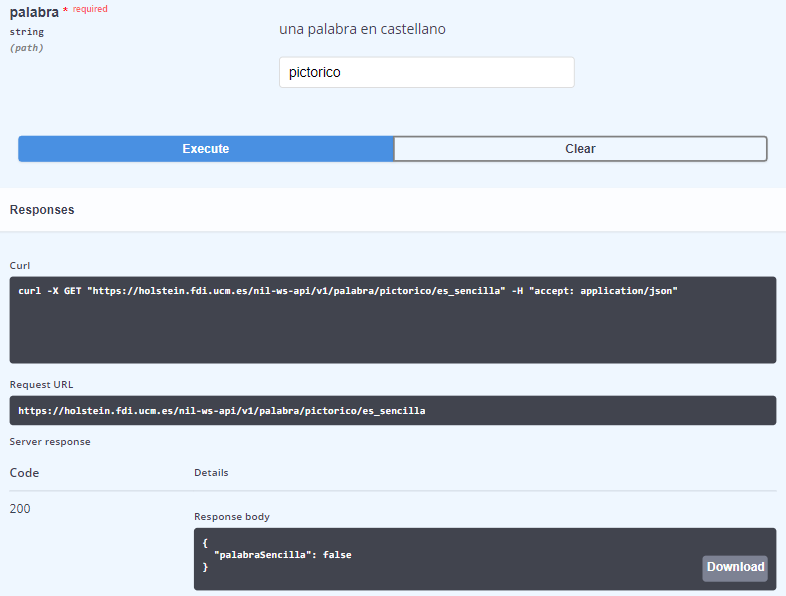
\includegraphics[scale=1]{Imagenes/Figuras/APISencilla}
		
		
		\caption{Petición para comprobar si una palabra es compleja}
		\label{fig:apiSencilla}
	\end{figure}
	\item \textbf{Servicio para obtener definiciones de una palabra}.


	\begin{lstlisting}[backgroundcolor = \color{pink},
	xleftmargin = 1cm,
	framexleftmargin = 1em,frame=tlbr,framesep=4pt,framerule=1pt]
	GET https://holstein.fdi.ucm.es/nil-ws-api/
	palabra/{palabra}/definiciones

	
	
\end{lstlisting}




En este caso, el servicio devuelve un objeto JSON que contiene el campo ``definiciones'' de tipo arrayList en el que en cada posición hay otro objeto ``definicion'' cuyo valor es de tipo string con la acepción correspondiente (ver Figura \ref{fig:apiDefinicion}).
\begin{figure}[h!]
	\centering
	
	
	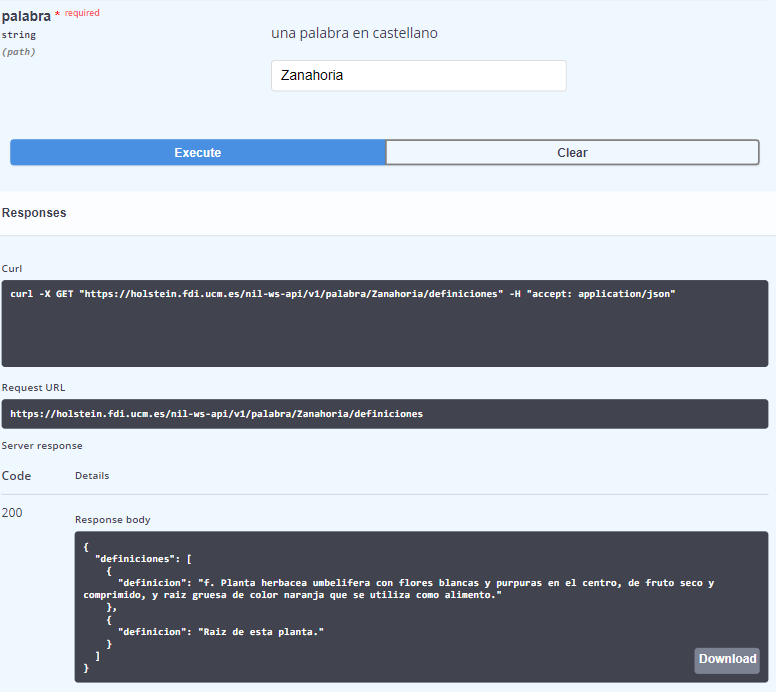
\includegraphics[scale=1]{Imagenes/Figuras/ApiDefinicion}
	
	
	\caption{Petición que devuelve una lista de definiciones}
	\label{fig:apiDefinicion}
\end{figure}
	\item \textbf{Servicio para obtener sinónimos de una palabra}.
	\begin{lstlisting}[backgroundcolor = \color{pink},
	xleftmargin = 1cm,
	framexleftmargin = 1em,frame=tlbr,framesep=4pt,framerule=1pt]
	GET https://holstein.fdi.ucm.es/nil-ws-api/
	palabra/{palabra}/sinonimos	
	
	
	
	
\end{lstlisting}



El servicio devuelve un objeto JSON que contiene el campo ``sinonimos'' de tipo arrayList en el que en cada posición hay otro objeto ``sinonimo'' cuyo valor es de tipo string con el sinónimo correspondiente (ver Figura \ref{fig:apiSinonimo}).
\begin{figure}[h!]
	\centering
	
	
	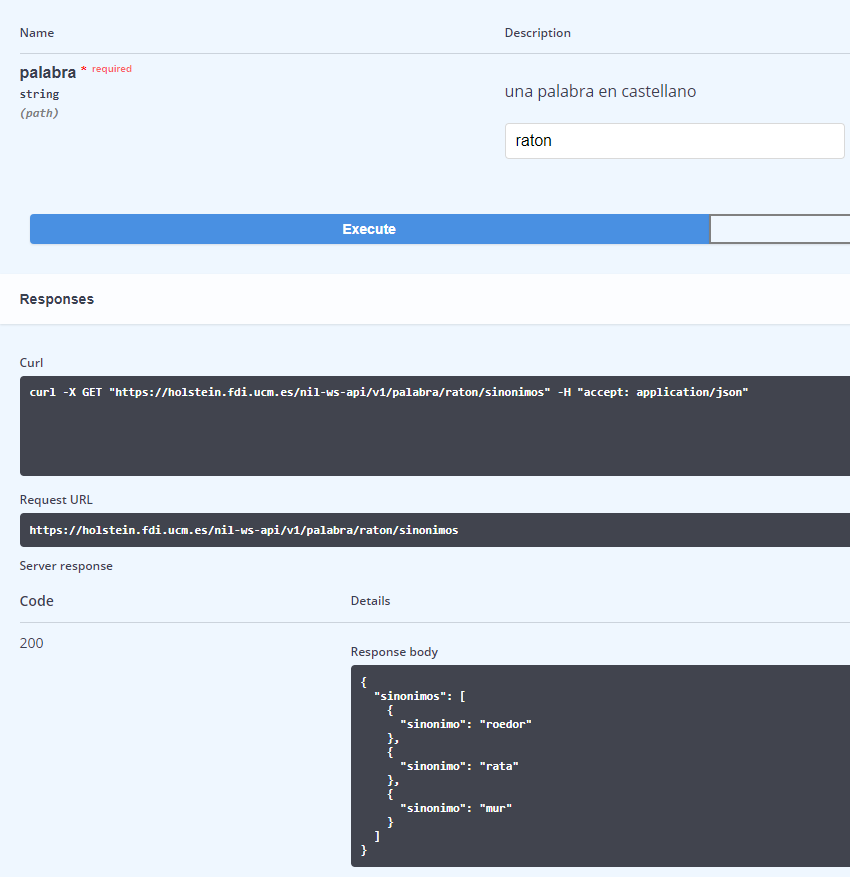
\includegraphics[scale=1]{Imagenes/Figuras/APISinonimos}
	
	
	\caption{Petición que devuelve una lista de sinónimos}
	\label{fig:apiSinonimo}
\end{figure}
\end{itemize}

Cabe destacar que esta API no hace uso de las reglas de acentuación, de manera que debemos de insertar las palabras sin tildes (obsérvese la Figura \ref{fig:apiSinonimo}, por ejemplo).

\subsection{Librería spaCy}\label{subsec:libreriaSpacy}

Para el procesamiento del lenguaje natural (PLN) nos hemos servido de la librería spaCy, en concreto para obtener el etiquetado gramatical y las dependencias entre las palabras de una frase (explicado en el capítulo \ref{cap:herramientas}, sección \ref{sec:spacy}).

El uso que damos a esta librería es muy similar en todos los endpoints utilizados en la aplicación, con la siguiente parte en común en cada función:
\begin{itemize}
	\item En primer lugar cargamos el modelo para procesar texto en español con el que vamos a trabajar. El código que se encarga de esto es el siguiente:
	\begin{lstlisting}[language=python,firstnumber=1]
		nlp = spacy.load("es_core_news_sm")
	\end{lstlisting}
\item Como segundo paso inicializamos el objeto spaCy a partir del lenguaje previamente elegido (español en nuestro caso) y del texto recibido (recibido previamente en formato JSON, obteniendo el valor que deseamos, en este caso el texto).
	\begin{lstlisting}[language=python,firstnumber=1]
	doc = nlp(text)
\end{lstlisting}
\end{itemize}


A continuación explicamos cómo y para qué hemos usado la librería spaCy en los diferentes endpoints:

\begin{itemize}
	\item \textbf{/isSimple}: este endpoint lo usamos para comprobar si las palabras de la frase son sencillas o complejas. A partir del objeto en formato spaCy obtenemos las etiquetas que marcan las categorías gramaticales del texto. Esto ha servido a la hora de filtrar las palabras para distinguir su gramática y poder excluir algunas, dado que no interesa saber si un signo de puntuación o un número se considera palabra sencilla o no, reduciendo la cantidad de llamadas a NIL-WS-API (/nil-ws-api/palabra/{palabra}/es\_sencilla), mejorando el tiempo de respuesta de este endpoint.
	
	\item \textbf{/summary}: para el uso de la funcionalidad ``resumen'', partiendo del objeto spaCy, conseguimos todas las palabras del texto, asignándoles una frecuencia de aparición. A continuación, obtenemos el texto dividido en frases mediante ``Sentence Boundary Detection'', que spaCy genera cuando creamos el objeto. A cada frase le asignamos una ``fuerza'' en función de cuantas palabras frecuentes (calculadas previamente) posea. De todas ellas, hacemos una selección del 40\% de las que tengan un valor mayor de ``fuerza''.
	
	\item \textbf{/sentences/tree}: este endpoint lo hemos usado para la construcción del árbol de dependencias. A partir del objeto spaCy obtenemos la palabra considerada raíz de la frase recibida. Esta será la referente de las que dependen las demás, generando así su árbol de dependencias con la función to\_nltk\_tree (para más aclaración ver sección \ref{subsec:implementacionesServidor}).
	
	\item \textbf{/sentences}: para obtener el texto dividido en frases, hacemos uso de este endpoint. Al generar el objeto spaCy reconoce automáticamente, a través de expresiones regulares, las frases que componen el texto.
\end{itemize}

\section{Implementaciones del servidor}\label{subsec:implementacionesServidor}

En esta subsección explicamos las principales funcionalidades implementadas en el servidor, los endpoints y las funciones auxiliares, con la finalidad de reducir la carga del navegador que ejecute la aplicación.

Parte de estas funcionalidades, implementadas en Python, han requerido el uso de servicios externos (explicados en la sección \ref{sec:serviciosWebExternos}) y la librería spaCy (explicada en la sección \ref{subsec:libreriaSpacy}). Las explicamos a continuación:

\begin{itemize}
	\item \textbf{isSimple}: es una función auxiliar que servirá de soporte a los endpoint ``/isSimple'' y ``/synonymous'', que realiza una petición GET al servicio NIL-WS-API (/nil-ws-api/palabra/<palabra>/es\_sencilla), devolviendo un booleano con valor ``TRUE'' en caso de que sea simple. En caso contrario, devolverá ``FALSE''.
	
	\item \textbf{simple}: función que se ejecutará desde la ruta ``/isSimple'', recibiendo un objeto JSON con una frase y recorriendo los tokens (palabras) que nos ha proporcionado spaCy usando la función auxiliar descrita en el primer punto. Así se genera una respuesta en formato JSON con un identificador de todas las palabras y un booleano que indican si son sencillas o no.
	
	\item \textbf{definition}: función que se realizará tras la llamada a la ruta ``/definition'', incluyendo un objeto JSON que contiene la palabra objeto de saber sus acepciones, y haciendo uso del servicio (/nil-ws-api/palabra/ <palabra>/definiciones) que nos proporciona NIL-WS-API.
	
	\item \textbf{summary}: funcionalidad que devuelve el resumen del texto, ya explicado en la sección \ref{subsec:libreriaSpacy}. Para llamar a esta función, se usa la ruta ``/summary''. 
	
	\item \textbf{to\_nltk\_tree}: A partir de un nodo (token) y la altura, inicialmente cero (nodo raíz), generamos de forma recursiva el árbol de dependencias con un recorrido en pre-orden, devolviéndolo completo.
	
	Cada nodo es de la clase personalizada \textbf{SentenceTree} localizada en el archivo vo.py, la cual tiene como atributos el texto del nodo, los hijos, la altura del nodo y un identificador único.
	
	\item \textbf{sentenceTree}: función encargada de generar el árbol de dependencias una vez se haya llamado a ``sentences/tree'', conteniendo este la función ``to\_nltk\_tree'. Se retorna un objeto JSON con la información del árbol de dependencias y un array que contiene cada palabra del árbol con su identificador para facilitar el procesado del mismo en la aplicación web.
	
	\item \textbf{splitTextInSentences}: función que genera la división del texto en frases. Estás se guardan en un array que se devuelve como un objeto JSON. Se accede a través de la ruta ``/sentences''.
	
	\item \textbf{synonymous}: función que se ejecuta con la llamada ``synonymous'' en la que se recibe, en formato JSON, la palabra. Eliminamos los signos de puntuación de la misma para poder hacer una llamada al servicio NIL-WS-API (/nil-ws-api/palabra/<palabra>/sinonimos) que devolverá la lista de sus sinónimos, si los tiene.
	Luego dividimos esa lista, llamando a la función ``isSimple'' por cada uno de ellos para saber si el sinónimo es sencillo o no, guardándolo en dos arrays distintos, que se devuelven como un JSON.
	
\end{itemize}

\section{Implementaciones de la aplicación web}\label{subsec:implementacionAplicacionWeb}

En esta sección se explica en detalle como han sido desarrolladas las funcionalidades (capítulo \ref{cap:asistenteWeb} sección \ref{sec:requisitosAplicacion}) desde un punto de vista de la interfaz. 

El archivo ``home.html'' inserta el de ``funciones.js'', desarollado en JavaScript, que será el encargado de llamar a los diferentes endpoints del servidor (archivo ``views.py''). Éste es el que nos proporcionará una respuesta que hará que modifique nuestra vista a través del DOM de una manera dinámica. A continuación, describimos los casos más importantes en los que se produciría este flujo:



\begin{itemize}
	\item Botón \textbf{Resumen}: se realiza una llamada Fetch al endpoint ``/summary''. Los datos a enviar en la petición POST  tienen la siguiente estructura JSON:
		\begin{lstlisting}
		
	         {"text": "<texto completo>"};
	
		
	\end{lstlisting}
	El campo ``text'' incluye el texto completo introducido previamente. La respuesta recibida será un objeto JSON, similar al siguiente:

	
		\begin{lstlisting}[language=json, firstnumber=1]
	{
		"summary": [
		"El Rastro de Madrid es el para|í|so de la nostalgia, un mercadillo |ú|nico que la pandemia ha puesto en la cuerda floja.",
		"La |ú|ltima apuesta para revitalizarlo es recuperar la Feria de desembalajes en la plaza del General Vara de Rey, una tradici|ó|n que tuvo su origen en los a|ñ|os 70, y que ahora se asienta el primer y el tercer s|á|bado del mes para dinamizar las ventas y que no se encasillen en los cl|á|sicos domingos."
		]
	}
		
	\end{lstlisting}
	El campo ``summary'' es un array en el que cada posición es una frase que constituye el resumen. Este array se recorre incrustándose cada frase en el código HTML a modo de lista (una debajo de otra). 
	
 
	\item Botón \textbf{Texto completo}: hacemos uso del endpoint ``/sentences'', devolviendo el texto completo en frases. La respuesta que nos da esta petición es la siguiente:
		\begin{lstlisting}[language=json, firstnumber=1]
{
	"sentences": [
	"Muebles antiguos, cuadros, l|á|mparas de vidrio, molinillos de caf|é|, porcelanas, vasijas, bustos y todo tipo de cachivaches.",
	"El Rastro de Madrid es el para|í|so de la nostalgia, un mercadillo |ú|nico que la pandemia ha puesto en la cuerda floja.",
	"Los comercios que viven de este enclave singular han pasado un a|ñ|o dif|í|cil, con bajos ingresos y muchas restricciones.",
	"Pero poco a poco, el Rastro vuelve a su ebullici|ó|n y reivindica la calle como un lugar de encuentro e intercambio.",
	"La |ú|ltima apuesta para revitalizarlo es recuperar la Feria de desembalajes en la plaza del General Vara de Rey, una tradici|ó|n que tuvo su origen en los a|ñ|os 70, y que ahora se asienta el primer y el tercer s|á|bado del mes para dinamizar las ventas y que no se encasillen en los cl|á|sicos domingos."
	]
}	
		\end{lstlisting}

    Al igual que en el caso anterior, haremos un recorrido en cada frase del array para mostrarlas en la interfaz de frases seleccionables en modo lista.
 
	
	\item \textbf{Creación y construcción del árbol de dependencias}: para esta parte hacemos una llamada Fetch al endpoint ``/sentences/tree''. El cuerpo de la petición POST incluirá el siguiente JSON:
	\begin{lstlisting}
		
		{"sentence": "<frase>"};
		
		
	\end{lstlisting}
	Lo que nos devuelve esta llamada son dos objetos JSON análogos, pero se van a usar para distintas finalidades. El primero, contendrá el campo ``sentencesIds'' siendo éste un array que incluirá un identificador único (campo ``id'') y la palabra (campo ``text''), que nos servirá para facilitar transformaciones futuras. Ese identificador es el mismo que se obtiene en la estructura del árbol, evitando así los problemas que puedan surgir con palabras duplicadas. Volcaremos el contenido en otro array de objetos al que llamaremos en referencias futuras ``sentenceArray'', que usaremos como soporte para cambiar dinámicamente el borrador del texto final, e iremos modificándolo en cada funcionalidad que requiera una transformación en el árbol de dependencias. Por ejemplo, para la frase ``La sonrisa es la mejor respuesta para una mirada.'', el JSON que recibimos tendría el siguiente aspecto: 
		\begin{lstlisting}[language=json,firstnumber=1]
	 "sentenceIds": [
	{
		"id": 0,
		"text": "La"
	},
	{
		"id": 1,
		"text": "sonrisa"
	},
	{
		"id": 2,
		"text": "es"
	},
	{
		"id": 3,
		"text": "la"
	},
	{
		"id": 4,
		"text": "mejor"
	},
	{
		"id": 5,
		"text": "respuesta"
	},
	{
		"id": 6,
		"text": "para"
	},
	{
		"id": 7,
		"text": "una"
	},
	{
		"id": 8,
		"text": "mirada"
	},
	{
		"id": 9,
		"text": "."
	}
	]
		
	\end{lstlisting}
	
	
	El segundo JSON que recibimos contiene la estructura del árbol, con los siguiente datos:
		\begin{itemize}
		\item \textbf{children}: array de nodos hijos.
		\item \textbf{height}: nivel del nodo con respecto a la raíz.
		\item \textbf{id}: identificador único de cada nodo.
		\item \textbf{text}: palabra propia del nodo.
	\end{itemize}
	Para la frase utilizada en el ejemplo anterior, el JSON recibido es: 
	
	\begin{lstlisting}[language=json,firstnumber=1]
		"tree": {
			"children": [
			{
				"children": [
				{
					"children": [],
					"height": 2,
					"id": 0,
					"text": "La"
				}
				],
				"height": 1,
				"id": 1,
				"text": "sonrisa"
			},
			{
				"children": [],
				"height": 1,
				"id": 2,
				"text": "es"
			},
			{
				"children": [],
				"height": 1,
				"id": 3,
				"text": "la"
			},
			{
				"children": [],
				"height": 1,
				"id": 4,
				"text": "mejor"
			},
			{
				"children": [
				{
					"children": [],
					"height": 2,
					"id": 6,
					"text": "para"
				},
				{
					"children": [],
					"height": 2,
					"id": 7,
					"text": "una"
				}
				],
				"height": 1,
				"id": 8,
				"text": "mirada"
			},
			{
				"children": [],
				"height": 1,
				"id": 9,
				"text": "."
			}
			],
			"height": 0,
			"id": 5,
			"text": "respuesta"
		}
	\end{lstlisting}

	
	Una vez tenemos la información para la construcción del árbol, se ha hecho uso de un algoritmo de búsqueda en profundidad (BFS)\footnote{Para más información  \href{https://es.wikipedia.org/wiki/B\%C3\%BAsqueda\_en\_profundidad}{https://es.wikipedia.org/wiki/B\%C3\%BAsqueda\_en\_profundidad}}, recorriendo todos los nodos (en nuestro caso palabras de la frase). El funcionamiento de este algoritmo consiste en ir expandiendo recursivamente cada uno de sus nodos desde la raíz hasta el nodo hoja, es decir, obedeciendo a la estructura del segundo JSON vamos procesando los arrays children de cada nodo hasta que este array sea vacío, insertando esos nodos en unas listas y sublistas en el HTML de manera recurrente. El flujo que se ha seguido para la implementación de este algoritmo se muestra en la Figura \ref{fig:diagramaBFS}.
	\begin{figure}[h!]
		\centering
		
		
		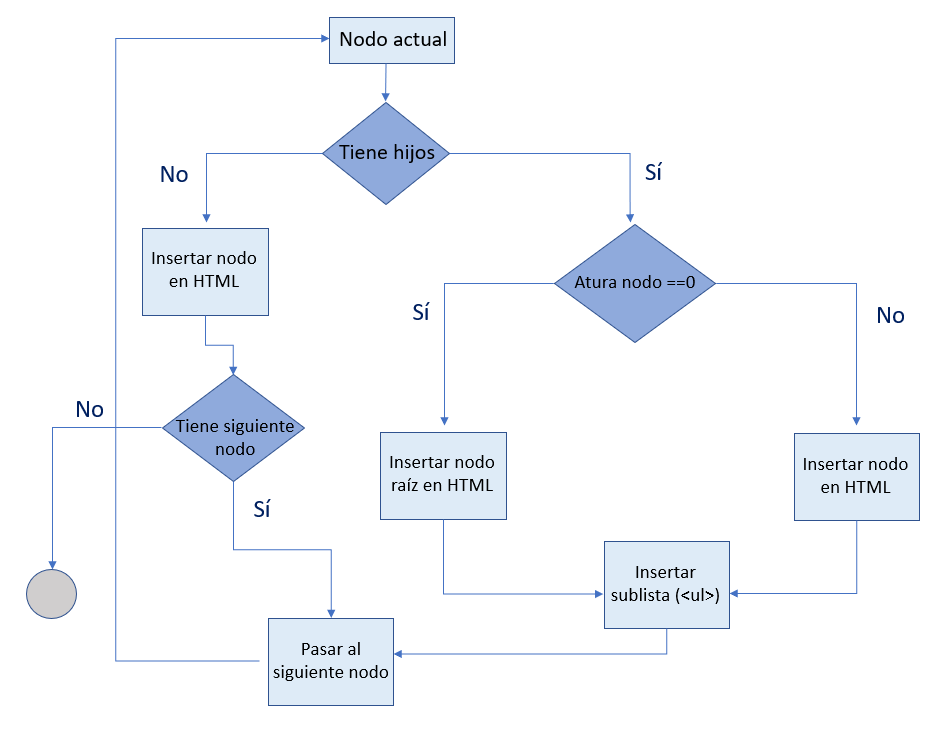
\includegraphics[scale=0.8]{Imagenes/Figuras/diagramaBFS}
		
		
		\caption{Diagrama de flujo de nuestro algoritmo BFS}
		\label{fig:diagramaBFS}
	\end{figure}
	
		\item Botón \textbf{Elección de las palabras}: cuando se hace clic en una palabra en el árbol de dependencias, se recoge su id, añadiéndole en el atributo classList la clase ``active'', que nos permite manipular el DOM de esa palabra. 
	\item Botón \textbf{Activar palabras complejas}: se realiza una petición POST al endpoint ``/isSimple'', con un objeto JSON, que contiene los siguientes datos:
		\begin{itemize}
		\item \textbf{id}: mismo identificador que se utiliza en la creación del árbol descrito anteriormente.
		\item \textbf{simple}: booleano con valor ``False'' si la palabra es compleja.
	
	\end{itemize}
		
Se recorre el objeto modificando los atributos en el DOM, en el caso de que la palabra (designada por su id) sea compleja, añadiendo una nueva clase para darle así un estilo destacado.
	
	\item Botón \textbf{Intercambio}: cuando se escogen dos palabras del árbol de dependencias, obtenemos sus ids gracias a la clase ``active''. Después se reemplaza en el DOM el id del primer término por el segundo y viceversa.
	Durante el desarrollo de esta parte hemos tratado la funcionalidad de dos maneras diferentes:
	\begin{itemize}
		\item Si las dos palabras son padre e hijo, se intercambia sólo sus ids y la palabra en el DOM, excluyendo sus dependencias.
		Para que se vea el resultado de este intercambio en el borrador final, se intercambia el contenido del ``sentenceArray'' de ambas palabras e ids.  
		\item Si el caso anterior no se da, se intercambian ambos nodos incluyendo los nodos dependientes, intercambiándolos en el DOM. En este caso, para escribir en el borrador la frase resultante, se guarda en un array auxiliar los ids involucrados, es decir, aquellos que formen parte de las palabras seleccionadas en el intercambio incluyendo estas y sus dependencias, ordenándolos de menor a mayor, para saber la posición inicial de dichos nodos. A continuación, se forma una sublista con los nodos de la primera palabra seleccionada y se extrae del array ``sentenceArray'' que se muestra a modo de ejemplo en la Figura \ref{fig:paso1y2}. Una vez eliminada esta sublista, se evalúa la nueva posición en la que se encuentra la segunda sublista y se vuelve a eliminar de ``sentenceArray'' como se puede ver en la Figura \ref{fig:paso3y4}. Por último se inserta la segunda sublista en la posición de la primera y viceversa (Figura \ref{fig:paso5}), teniendo así nuestra frase con este intercambio en el array ``sentenceArray'' como observamos en la Figura \ref{fig:paso6}.
			\begin{figure}[h!]
			\centering
			
			
			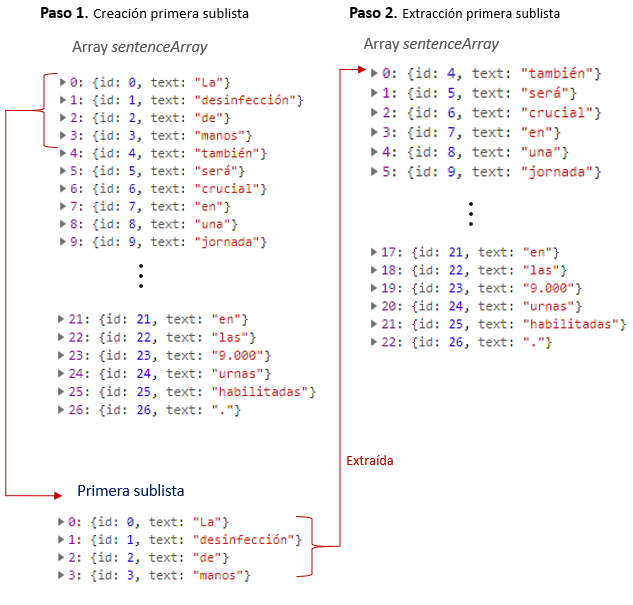
\includegraphics[scale=1.2]{Imagenes/Figuras/IntercambioPaso1_y_2}
			
			
			\caption{Creación y extracción de la primera sublista del array ``sentenceArray''.}
			\label{fig:paso1y2}
		\end{figure}
		\begin{figure}[h!]
		\centering
		
		
		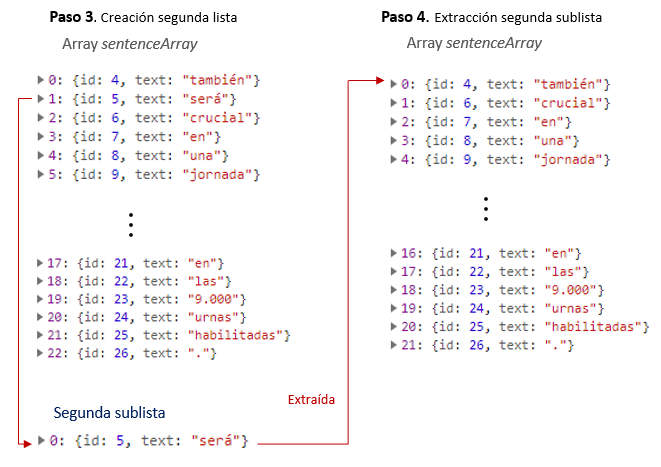
\includegraphics[scale=1.1]{Imagenes/Figuras/IntercambioPaso3_y_4}
		
		
		\caption{Creación y extracción de la segunda sublista del array ``sentenceArray''.}
		\label{fig:paso3y4}
	\end{figure}
	\begin{figure}[h!]
	\centering
	
	
	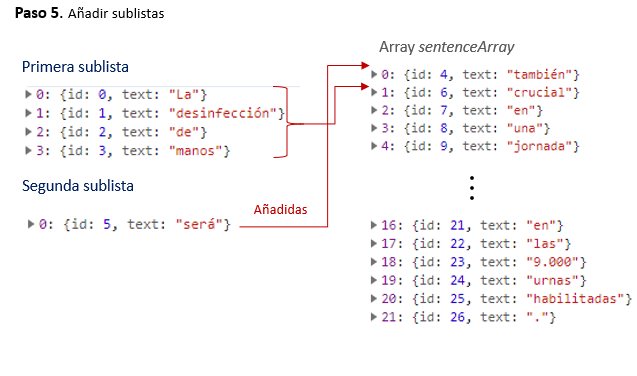
\includegraphics[scale=1.1]{Imagenes/Figuras/IntercambioPaso5}
	
	
	\caption{Inserción de ambas sublistas en el array ``sentenceArray''.}
	\label{fig:paso5}
\end{figure}
	\begin{figure}[h!]
	\centering
	
	
	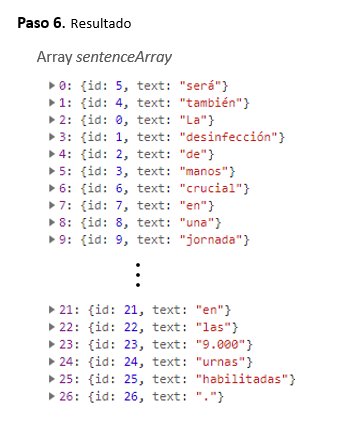
\includegraphics[scale=1.3]{Imagenes/Figuras/IntercambioPaso6}
	
	
	\caption{Resultado del array ``sentenceArray'' tras el intercambio.}
	\label{fig:paso6}
\end{figure}

		
	
	\end{itemize}

	\item Botón \textbf{Sinónimos}: antes de la llamada al endpoint correspondiente (``/synonymous''), la palabra seleccionada será convertida a un objeto JSON de la siguiente manera:
	\begin{lstlisting}
	       
	        objeto = {"synonymous": "Mirada"}
	        jsonObj = JSON.stringify(objeto);
	
	\end{lstlisting}
	Tras la llamada, se recibirá una respuesta con dos objetos JSON, uno con un listado de sinónimos sencillos, si los tiene, y otro con los complejos. Si la palabra no tuviese sinónimos, una de las listas o ambas serán vacías:
		\begin{lstlisting}[language=json,firstnumber=1]
		{
		"simpleSynonymous": [],
		"synonymous": [
						"ojeada",
						"vistazo",
						"observacion",
						"inspeccion",
						"examen"
						]
	}
	\end{lstlisting}
	


	Para introducir los sinónimos en HTML se recorren ambos objetos, siempre y cuando tengan algún sinónimo, y se van incrustando en HTML con la etiqueta de lista (no enumerada). En este caso, observamos en el código de ejemplo anterior que la palabra ``Mirada'' no nos devuelve sinónimos sencillos (campo ``simpleSynonymous''), mostrando una lista vacía. En cambio, sí que podremos observar una lista de sinónimos complejos (campo ``synonymous'').
	
	En este endpoint encontramos un inconveniente. En ocasiones, los sinónimos recibidos no concuerden correctamente en número, persona o conjugación con el contexto de la frase. Para solucionarlo, hemos optado por que el usuario pueda ser capaz de editarlo in situ. Así, en la lista de los sinónimos cada uno tendrá un input que se mostrará con el botón que aparece a su derecha para editarlo. Se recogerá el valor del input modificándolo en el DOM.
	

	\item Botón \textbf{Eliminar}: esta funcionalidad se ha realizado tomando de nuevo el id asociado a la palabra seleccionada de nuestro árbol mediante la clase ``active''. Para eliminar una palabra o subárbol, es decir, palabra propia seleccionada y sus dependientes en el borrador final, necesitaremos la ayuda de un array auxiliar, donde almacenamos todos los ids que dependen de la palabra, incluida ésta, ordenándolos de forma creciente. Como hemos visto en la construcción del árbol, tenemos a nuestra disposición el ``sentenceArray'' con el id y la palabra, asociados entre sí, que vamos a usar para extraer el contenido del array auxiliar en el ``sentenceArray''  para escribir el resultado en el borrador. Para hacer esta eliminación en el árbol se hace uso del ChildNode.remove(), que proporciona JavaScript para eliminar el objeto del DOM al que pertenece.




	\item Botón \textbf{Definición}: se realiza una llamada Fetch al endpoint ``/definition'' con el siguiente JSON:
		\begin{lstlisting}
		
		{"word": "<palabra>"}
		
		
	\end{lstlisting}
	
	 El resultado de la petición consistirá en un objeto JSON con un listado de las acepciones, si las tiene, y en caso contrario devolverá una lista vacía. El siguiente código muestra el resultado una vez realizada la petición POST con la palabra ``secador'':
	 	\begin{lstlisting}[language=json,firstnumber=1]
	 	{
	 		"definiciones": [
	 		{
	 			"definicion": "adj. Que seca."
	 		},
	 		{
	 			"definicion": "m. y f. Aparato o maquina que sirve para secar."
	 		}
	 		]
	 	}
	 \end{lstlisting}
	Estas definiciones se insertan en el código HTML, escribiéndolas a modo de lista, incluyendo un enlace para seleccionarlas y poder adjuntarlas al borrador.    
	




\end{itemize}


\section{Extensibilidad del asistente web interactivo}
Una vez explicada la implementación tanto la parte relacionada con el servidor como de la aplicación en sí, describiremos a continuación qué pasos debe de seguir un desarrollador que retome este asistente y desee añadir una nueva funcionalidad que requiera del uso de los servicios que ofrece NIL-WS-API o la librería spaCy.

Para ello, habría que realizar modificaciones en los siguientes ficheros:
\begin{itemize}
	\item \textbf{views.py}: en el caso de que sea necesario añadir una nueva funcionalidad llamando a un servicio de NIL-WS-API mediante un nuevo endpoint. He aquí un ejemplo:
	
			\begin{lstlisting}[language=python,firstnumber=1]
	@app.route('/definition', methods=['POST'])
	def definition():
	word=request.get_json()
	word=word['word']
	response = requests.get(NILWS_URL + word + DEFINITION_URL)
	data = response.json()
	
	return jsonify(definiciones=data['definiciones'])
	\end{lstlisting}

Aspectos a tener en cuenta para llamar a un servicio NIL-WS-API:
\begin{itemize}
	\item En la línea 1 se escribirá la instrucción ``$@$app.route('<ruta>', methods=['POST'])'' con el endpoint correspondiente. Esta instrucción se utilizará para llamar a la ruta desde funciones.js.
	\item En la línea 2 se define el nombre de la función.
	\item En la línea 3 convierte el objeto JSON de la petición en datos de Python para utilizarlos a la hora de enviar la petición en la línea 5.
	\item En la línea 5 se realiza la llamada al servicio NIL-WS-API guardando su respuesta.
	\item En las líneas sucesivas se produce el tratamiento de la respuesta a esa petición.
\end{itemize}

A la hora de utilizar la librería spaCy, cabe destacar que:

\begin{itemize}
	\item Las cuatro primeras líneas tienen el mismo comportamiento que las de una petición de un servicio de la API.
	\item En la línea 5 cargamos un modelo para procesar texto en español.
	\item En la línea 6 se ejecuta una llamada a nlp para producir un documento analizado.
	\item En las líneas posteriores se procederá a la manipulación de este documento.
\end{itemize}

\begin{lstlisting}[language=python,firstnumber=1]
	@app.route('/sentences/tree', methods=['POST'])
	def sentenceTree():
	data = request.get_json()
	sentence = data["sentence"]
	nlp = spacy.load("es_core_news_sm")
	doc = nlp(sentence)
	{...} #Tratamiento del documento.
\end{lstlisting}

	
	\item \textbf{funciones.js}: en este fichero se añade una nueva función que incluya una llamada Fetch mandando los diferentes campos para el uso de una ruta determinada que se llamará en views.py. 
	
	\begin{lstlisting}[language=python,firstnumber=1]
	function definition() {
		{...}
		
		var j = {"word": palabra}
		var jsonObj = JSON.stringify(j);
		fetch("/definition", {
			method: "POST",
			headers: {
				'Content-Type': 'application/json',
			},
			body: jsonObj
		}).then(response => response.json()
		).then(data => {
			var elements = data.definiciones;
			
		{...} //Operaciones a realizar tras la respuesta.
			
		}
		);		
	}
	\end{lstlisting}
	
	
	
	
	
	\item \textbf{home.html}: añadir un nuevo componente a la interfaz que se encargue de llamar a una función del archivo ``funciones.js''. 
		\begin{lstlisting}[language=python,firstnumber=1]
	<button title="Consulta la/s definici|ó|n/es de una palabra del |á|rbol seleccionada"
	id="bDefinicion" class="botonesFuncionales" disabled
	onclick="definition();">Definici|ó|n
	</button>
	\end{lstlisting}
	\item \textbf{styles.css}: añadir nuevas reglas para dar estilo al nuevo componente de la vista objeto de la nueva funcionalidad (colores, tamaños, etc.)
\end{itemize}
